\section{Resolución Problema 3}
\subsection{Problema:}
Dada una circunferencia con centro en el punto $C$ con coordenadas $(x_{1}, y_{1})$ y radio $r$, evaluar si un punto $T$ con coordenadas $(x_{2}, y_{2})$ esta dentro del area de la circunferencia.

\subsection{\textbf{Descripción del problema:}}

El problema consiste en determinar si un punto $T$, dado por sus coordenadas $(x_{2}, y_{2})$, se encuentra dentro de la aérea de una circunferencia específica. Esta circunferencia está definida por su centro, ubicado en el punto $C$ con coordenadas $(x_{1}, y_{1})$, y su radio, que es una medida determinada.

\begin{figure}[h!]
    \centering
    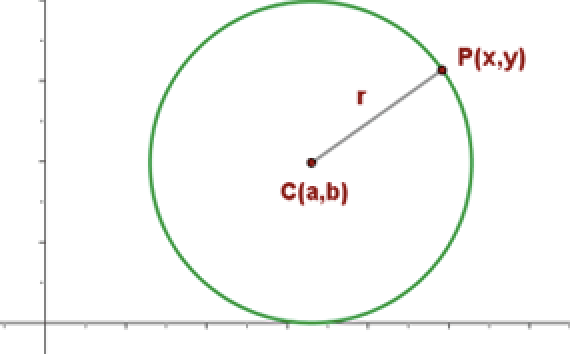
\includegraphics[width = 4 cm]{LaTeX/latex-imagenes/circunferenciaE3.png}
    \caption{Circunferencia con dos puntos a distancia.}
    \label{fig:uno}
\end{figure}


\subsection{\textbf{Definición de solución:}}

La solución para evaluar este problema implica utilizar la fórmula de la distancia euclidiana, es la fórmula más común para calcular la distancia entre dos puntos. Esta fórmula se basa en el teorema de Pitágoras y es válida para puntos en un plano euclidiano.

La distancia se calcula como la raíz cuadrada de la suma de los cuadrados de las diferencias entre las coordenadas $x$ y las coordenadas $y$ de ambos puntos:
\begin{equation}
Distancia = 
   \sqrt{ (x_2 - x_1)^2 + (y_2 - y_1)^2 }     
\end{equation}

\par Por ejemplo, si tenemos dos puntos $A$ (2,3) y $B$ (5,7), podemos usar la fórmula de distancia euclidiana para calcular su distancia:\\

\begin{figure}[h!]
    \centering
    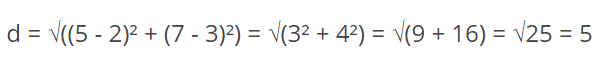
\includegraphics[width = 8 cm]{LaTeX/latex-imagenes/Ejemplo E3.png}
    \caption{Por lo tanto, la distancia entre Ay B es de 5 unidades}
    \label{fig:Ejemplo}
\end{figure}


Al final solo comparamos la distancia calculada con el radio $r$ de la circunferencia:

\begin{itemize}
\renewcommand\labelitemi{--}
\item Si la distancia es mayor que el radio $r$, el punto $T$ está fuera de la circunferencia.
\item Si la distancia es igual al radio $r$, el punto $T$ está en el borde de la circunferencia.
\item Si la distancia es menor que el radio $r$, el punto $T$ está dentro del área de la circunferencia.\\    
\end{itemize}

\begin{figure}[h!]
    \centering
    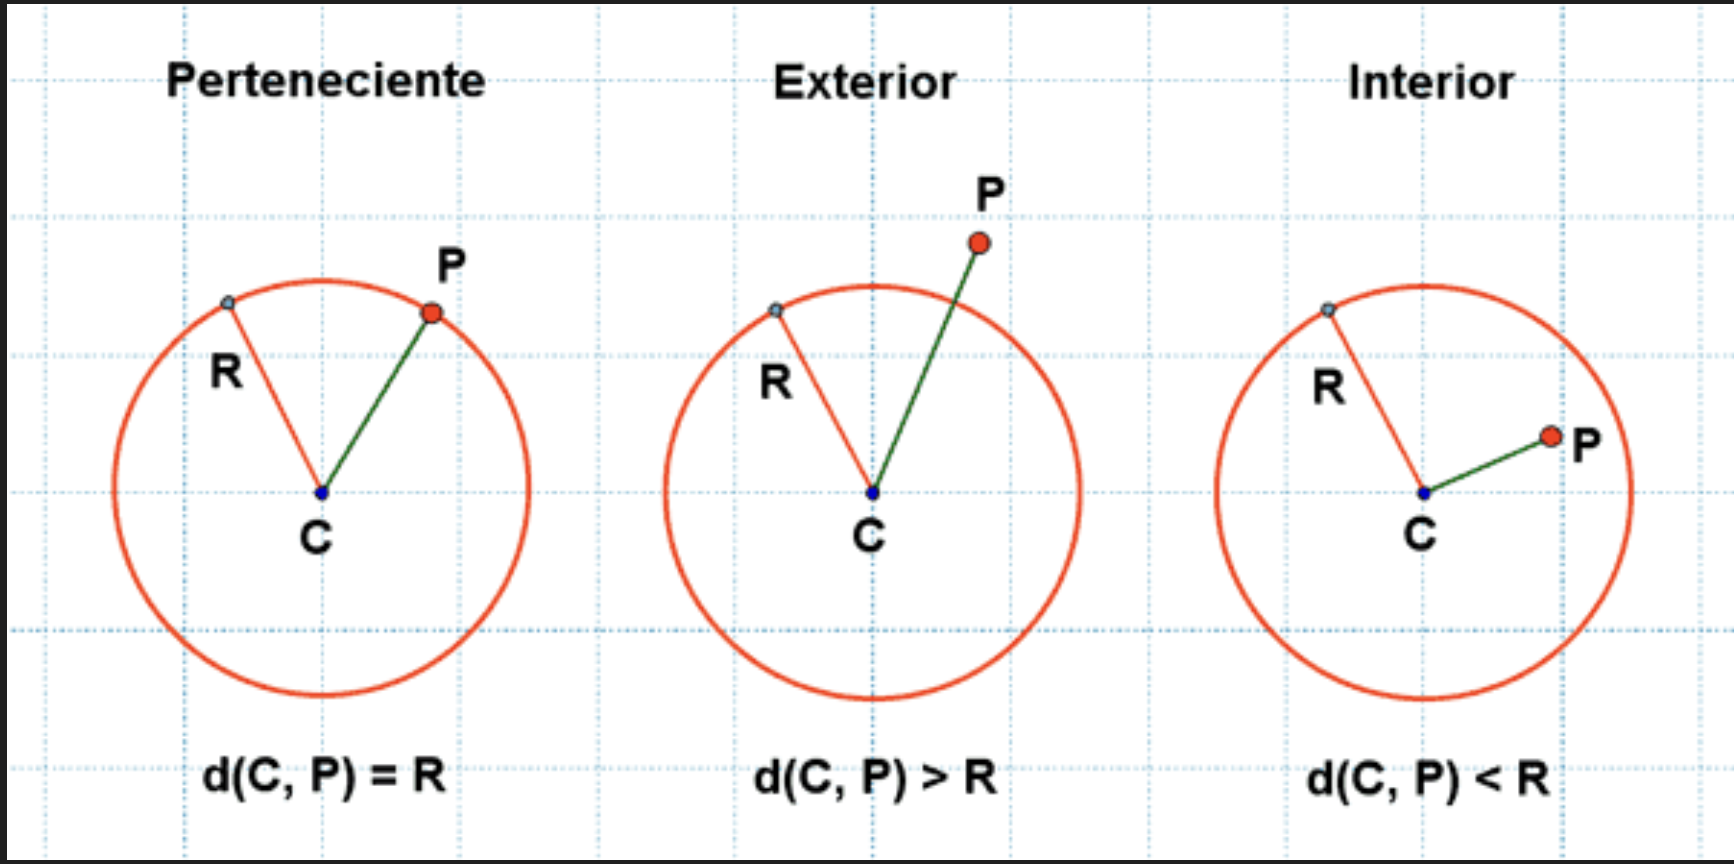
\includegraphics[width = 5 cm]{LaTeX/latex-imagenes/circunferenciaE32.png}
    \caption{Ejemplo de comparación de la distancia y el radio.}
    \label{fig:uno}
\end{figure}


\subsection{\textbf{Diseño de la solución:}}

\begin{enumerate}
\item Solicitar al usuario que ingrese las coordenadas del punto $C$ y el punto $T$, es decir $(x_{1}, y_{1})$ y $(x_{2}, y_{2})$ y el radio $r$.
\item Calcular la distancia entre el centro y el punto.
\item Verificar si el punto está dentro del área de la circunferencia
\item Al final mostrar el resultado al usuario \\
\end{enumerate}

\begin{figure}[h!]
    \centering
    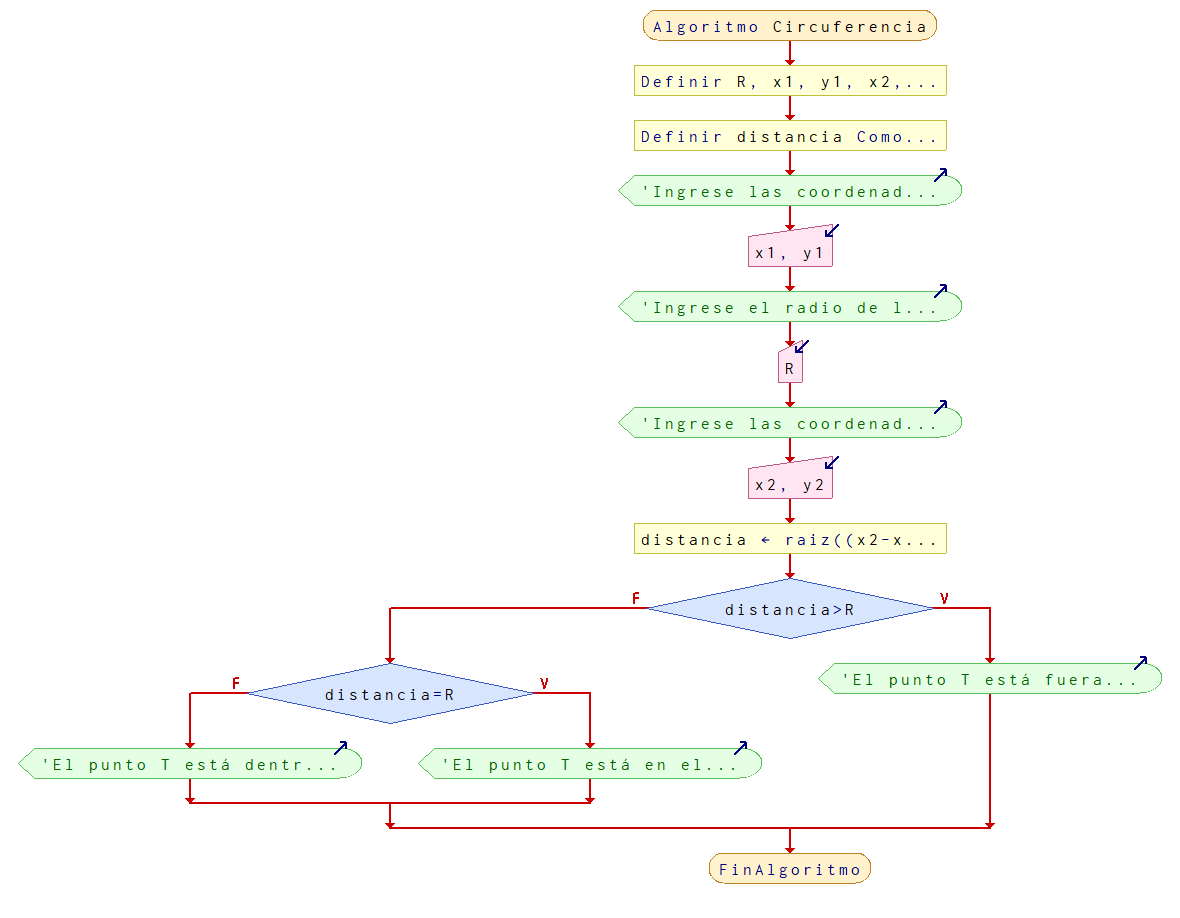
\includegraphics[width = 8 cm]{LaTeX/latex-imagenes/DiagramaE3.png}
    \caption{Diagrama de flujo del problema 3}
    \label{fig:DiagrmadeFlujo}
\end{figure}


\subsection{\textbf{Desarrollo de la solución:}}

Se importa la clase Scanner para que se pueda leer las entradas del usuario
\begin{lstlisting}[style=javaStyle]
import java.util.Scanner;
\end{lstlisting}

Posteriormente se define la clase llamada "CircufrenciaIntegrador" que contendrá el programa.
\begin{lstlisting}[style=javaStyle]
    public class CircuferenciaIntegrador {
    public static void main(String[] args) {} 
\end{lstlisting}\\

Igualmente se crea una instancia de Scanner para leer la entrada del usuario
\begin{lstlisting}[style=javaStyle]
Scanner datC = new Scanner(System.in);
\end{lstlisting}

Se solicita al usuario que ingrese las coordenadas del punto C en el formato \textbf{"x1, y1"}, las cuales se almacenan en un arreglo de cadenas llamado \textbf{"puntoC"}
\begin{lstlisting}[style=javaStyle]
System.out.print("""
                Ingrese las coordenadas del punto C 
                seperadas por una coma (x1, y1):
                         """);
    String[] puntoC = (datC.nextLine()).split(",");
\end{lstlisting}

Igualmente se solicita al usuario que ingrese el $radio$ de la circunferencia, se almacena en una variable $r$ de tipo float
\begin{lstlisting}[style=javaStyle]
System.out.print("Ingrese el radio de la circunferencia: ");
    float r = datC.nextFloat();
    datC.nextLine();  
\end{lstlisting}

Seguidamente se solicita al usuario que ingrese las coordenadas del punto T que es el punto de , en el formato \textbf{"x2, y2"} que se almacenan en un arreglo de cadenas llamado \textbf{"puntoT"}
\begin{lstlisting}[style=javaStyle]
//Obtener las coordenadas del punto a verificar
System.out.print("""
                Ingrese las coordenadas del punto T
                seperadas por una coma (x2, y2): 
                         """);
String[] puntoT = (datC.nextLine()).split(",");
\end{lstlisting}

Se Cierra el objeto Scanner para liberar los recursos.
\begin{lstlisting}[style=javaStyle]
                  datC.close(); 
\end{lstlisting}
Se convierte las coordenadas del punto C y del punto T de cadenas a enteros (x1, y1, x2, y2).
En Java, convertir datos en cadenas a enteros es útil cuando necesitas manipular o realizar operaciones matemáticas con números enteros que se encuentran representados como \textit{cadenas de caracteres}.
\begin{lstlisting}[style=javaStyle]
int x1 = Integer.parseInt(puntoC[0].trim());
int y1 = Integer.parseInt(puntoC[1].trim());
        
int x2 = Integer.parseInt(puntoT[0].trim());
int y2 = Integer.parseInt(puntoT[1].trim());
\end{lstlisting}

En esta parte del desarrollo se calcula la distancia entre el centro (punto C) y el punto T utilizando la fórmula de la distancia euclidiana que significa; la distancia en línea recta entre dos puntos en un plano.
\begin{lstlisting}[style=javaStyle]
float distancia = (float)Math.sqrt(Math.pow(x2 - x1, 2) + Math.pow(y2 - y1, 2));   
\end{lstlisting}

Al final se utiliza las condiciones \textbf{if, else if y else} para evaluar la relación entre la distancia y el radio de la circunferencia, con esto se verifica si el punto T se encuentra dentro de la circunferencia, en el borde o fuera de ella y se muestra el resultado al usuario.
\begin{lstlisting}[style=javaStyle]
//Verificar si el punto está dentro del área de la circunferencia
     if (distancia > r) {
    System.out.println("El punto T("+x2+","+y2+") esta fuera de la circunferencia");
    }else if (distancia == r) {
     System.out.println("El punto T("+x2+","+y2+") esta en el borde de la circunferencia");
    }else if (distancia < r){
     System.out.println("El punto T("+x2+","+y2+") esta dentro de la circunferencia"); }
\end{lstlisting}

\subsection{\textbf{Depuración y pruebas:}}

\begin{table}[h!]
     \centering
     \caption{Tabla de Corridas del problema 3}\\

     \begin{tabular}{|c|c|c|c|c|c|}
     \hline
    Corrida & C$(x_{1}, y_{1})$& T$(x_{2}, y_{2})$  &  R $r$ & Resultado\\
    \hline
    1  &  $(3,4)$ & $(9,2)$ & 10 & $T$ esta adentro \\
    \hline
    2  &  $(5,2)$ & $(8,1)$ & 12 & $T$ esta adentro \\
    \hline
    3  &  $(34,23)$ & $(-90,35)$ & 67 & $T$ esta afuera \\
    \hline
    4  &  $(-27,3)$ & $(34,-5)$ & 30 & $T$ esta afuera \\
    \hline
    5 &  $(2,8)$ & $(4,9)$ & 17 & $T$ esta adentro \\
    \hline
     \end{tabular}
     \label{tab:my_label}
 \end{table}
